\RequirePackage[T1]{fontenc}
\documentclass[10pt,journal,twoside]{IEEEtran}
\usepackage{amsmath,amssymb,graphicx,booktabs,array,cite,placeins}
\usepackage[ruled,vlined,linesnumbered]{algorithm2e}
\usepackage[hidelinks]{hyperref}
\graphicspath{{figures/}}
\newcommand{\ee}{\mathbf e}
\newcommand{\nn}{\mathbf n}
\newcommand{\pp}{\mathbf p}
\newcommand{\hh}{\mathbf h}
\newcommand{\qq}{\mathbf q}
\newcommand{\RR}{\mathbf R}
\newcommand{\xx}{\mathbf x}
\newcommand{\argmin}{\mathop{\mathrm{arg\,min}}}
\newtheorem{proposition}{Proposition}
\newtheorem{theorem}{Theorem}
\hyphenation{non-holonomic com-ple-men-tarity quad-ru-ped}
\setlength{\emergencystretch}{1em}
\setlength{\textfloatsep}{8pt plus 2pt minus 2pt}
\setlength{\dbltextfloatsep}{8pt plus 2pt minus 2pt}
\setlength{\floatsep}{7pt plus 2pt minus 2pt}
\setlength{\abovecaptionskip}{2pt}
\setlength{\belowcaptionskip}{0pt}
\setlength{\abovedisplayskip}{5pt plus 1pt minus 1pt}
\setlength{\belowdisplayskip}{5pt plus 1pt minus 1pt}
\renewcommand{\dbltopfraction}{.88}
\renewcommand{\topfraction}{.90}
\renewcommand{\textfraction}{.08}
\setcounter{dbltopnumber}{2}
\setcounter{topnumber}{4}
\setcounter{totalnumber}{6}
\makeatletter
\setlength{\@fptop}{0pt}
\setlength{\@fpsep}{8pt}
\setlength{\@fpbot}{0pt plus 1fil}
\setlength{\@dblfptop}{0pt}
\setlength{\@dblfpsep}{8pt}
\setlength{\@dblfpbot}{0pt plus 1fil}
\makeatother
\title{Optimization-Based Motion Planning for Autonomous Cable-Towing Vehicles in Confined Warehouses}
\author{Anonymous manuscript}
\hypersetup{pdftitle={Optimization-Based Motion Planning for Autonomous Cable-Towing Vehicles in Confined Warehouses},pdfauthor={}}
\markboth{IEEE Transactions on Automation Science and Engineering (Manuscript)}{Optimization-Based Planning for Autonomous Cable Towing}
\begin{document}
\raggedbottom
\newcommand{\ProposedNew}{9/9}
\newcommand{\ProposedGain}{4.36}
\newcommand{\MaxNew}{8/9}
\newcommand{\MaxGain}{0.97}
\newcommand{\ProposedTime}{31.03}
\newcommand{\MaxTime}{30.97}

\maketitle
\begin{abstract}
An autonomous warehouse tractor can create cable slack, reposition while its passive cart waits, and resume pulling from a different direction. This paper develops optimization-based motion planning for this transport under quasistatic stopping and hitch-mobility assumptions. A six-state model combines first-order Euler updates with a direct maximum describing slack--taut transmission. A geometric barrier excludes rigid articulated reorientation in a specified strip family; numerical cable trajectories satisfy the discrete model and geometric routing checks in 18 corresponding tasks. For feasible-seed trajectory refinement, relaxed initialization and control restoration guide direct-max optimization with optimization-based collision avoidance (OBCA). Replay-derived clearance reserves improve refinement under integration drift, while independent replay determines final acceptance. Comparisons transfer published towing strategies into common models, seeds, and computational allowances. Across nine warehouse tasks, the proposed method produces \ProposedNew{} new validated outputs and reduces mean per-case tractor travel by \ProposedGain\%, compared with \MaxNew{} and \MaxGain\% for direct maximum. Median backend times are \ProposedTime{} s and \MaxTime{} s. Controlled ablations attribute the quality gains to the combined refinement stages. Five cart footprints and a constructive three-cart example extend the geometric evaluation.
\end{abstract}

\vspace{.3em}
{\small
\noindent\textbf{Note to Practitioners---}A warehouse can concentrate propulsion, sensing, and planning in one autonomous tug while using passive carts with different load outlines. Cable connections support temporary transport formations and let the tug reposition while a loaded cart waits. The cable length remains fixed; slack accommodates changes in endpoint separation without a telescopic mechanism. This freedom is useful near rack ends, transfer gates, and loading pockets, where moving the load merely to turn the tug consumes space. The proposed optimization-based planner refines a feasible transport route before task execution, accounts for complete vehicle shapes, and checks geometric cable routes. A validated trajectory remains available throughout refinement. The intended operation is low-speed transport on a known map with sufficient resistance for rapid stopping of an unpulled cart. The simulated tasks target arrival regions for warehouse transfers. Deployment will require verification of the stopping and hitch-mobility assumptions, continuous cable handling, and trajectory tracking on the physical platform.
\par}

\vspace{\baselineskip}
\begin{IEEEkeywords}
Cable towing, autonomous vehicles, warehouse logistics, optimization-based motion planning, hybrid kinematics, nonlinear optimization.
\end{IEEEkeywords}
\section{Introduction}
\IEEEPARstart{A}{utonomous} warehouse transport must fit the geometry of racks, transfer gates, and loading pockets as well as the load capacity of vehicles. In confined aisles, changing orientation requires clearance for the complete tractor and payload. Recent studies in this journal improve tractor--trailer planning~\cite{xu2025,gatro2026}, generalized trailer trains~\cite{deniz2025}, motion representations~\cite{ddr2025}, and coordinated transport in dense environments~\cite{xu2024dense}. These advances also motivate a mechanical question: can a different connection make a previously obstructed maneuver possible?

A rigid vehicle carries its load in one body. A conventional articulated vehicle separates the tractor and payload, joined by a fixed drawbar. An inextensible cable permits an additional maneuver: the tractor can move toward the payload, create slack, and reposition while the payload remains stationary. Pulling resumes as the cable becomes taut. The material length stays fixed; the endpoint separation changes through cable bending. Figure~\ref{fig:warehouse} illustrates this operation near warehouse racks.

\begin{figure*}[!t]
\centering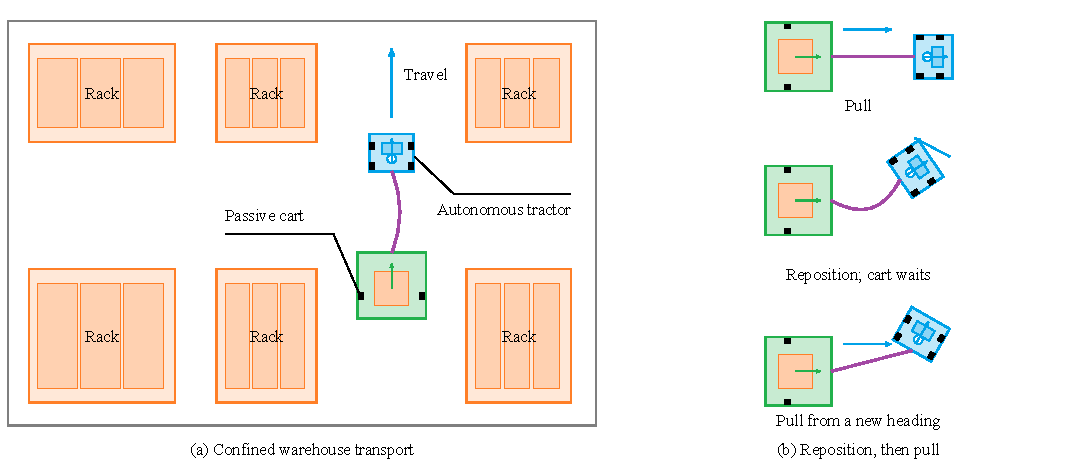
\includegraphics[width=\textwidth]{warehouse_concept.pdf}
\caption{Single-cart cable towing and tractor repositioning in a confined warehouse.}
\label{fig:warehouse}
\end{figure*}

The system comprises an autonomous car-like tractor and passive wheeled trailers, termed \emph{carts} hereafter. Propulsion, perception, planning, and tracking are concentrated in the tractor. A cable connection accommodates temporary formations and different cart outlines, while allowing the tractor to reposition independently of a waiting load. We study low-speed transport under a quasistatic mobility model: an unpulled cart stops immediately, and a pulled front hitch moves along the cable direction. These operating assumptions define the passive-cart class considered here. The resulting optimization-based planner prepares transport trajectories before task execution, starting from a feasible control sequence.

Cable towing has related precedents in leash-guided interaction~\cite{xiao2021}, collaborative quadruped towing~\cite{yang2022}, heterogeneous robot transport~\cite{xu2024cable}, and a quadruped towing a wheeled cart~\cite{zhang2026}. The present problem combines a curvature-bounded autonomous tractor, nonreversing passive carts, convex polygonal footprints, and repeated slack--taut transitions. Different payload outlines therefore change the feasible tractor motion.

Two questions organize the study. First, does cable coupling enable maneuvers excluded by a standard rigid drawbar with the same body geometry and length? Second, within the same cable system, which numerical strategy offers better trajectory quality, acceptance, and computation time? The contributions address these questions separately:
\begin{enumerate}
\item A six-state kinematic formulation combines Euler updates with a unilateral cable endpoint closure, supports convex polygonal footprints of arbitrary shape through optimization-based collision avoidance (OBCA)~\cite{obca2021}, and propagates recursively along serial carts. A geometric theorem identifies a rigid-coupling obstruction; corresponding cable trajectories are validated under the discrete model and geometric routing checks.
\item An optimization-based method for feasible-seed trajectory refinement combines relaxed initialization, feasible control restoration, replay-guided clearance reserves, and final recovery. Equivalent mode formulations and strategies adapted from published towing studies are compared under common models, maps, initial trajectories, and validation rules. Matched ablations isolate the numerical mechanisms.
\end{enumerate}

\section{Related Work}
Articulated transport provides the mechanical baseline, cable-connected systems motivate mode strategies, and hybrid optimization provides tools for their numerical treatment.

\subsection{Articulated Vehicles and Warehouse Automation}
Articulated planning couples nonholonomic motion, multiple body footprints, and successive headings. Ljungqvist et al.~\cite{ljungqvist2019} combine planning and tracking for a general two-trailer vehicle. Deniz and Auat Cheein~\cite{deniz2025} develop predictive path-following for generalized trailer trains with dynamic obstacles. Tracailer~\cite{xu2025} integrates a compact smooth trajectory representation with efficient initial-path search. GATRO~\cite{gatro2026} exploits semidefinite structure and graphics processing unit (GPU) acceleration. These methods advance rigid-coupling transport; flexible connections introduce additional relative configurations and switching behavior.

Broader warehouse and mobile-robot studies address complementary issues. Bidirectional--unidirectional sampling~\cite{wang2022rrt} improves difficult kinodynamic connections, while dense-environment coordination~\cite{xu2024dense} couples task assignment with motion. Learned parking trajectories~\cite{chai2023} and two-stage coverage optimization~\cite{painting2025} illustrate the role of initial solutions and discrete decisions. Universal differential-drive planning~\cite{ddr2025} and spatial--temporal planning for car-like robots~\cite{han2024} emphasize representations matched to platform constraints. Our numerical study fixes those constraints and compares cable-mode handling.

\subsection{Cable-Connected Transport}
Xiao et al.~\cite{xiao2021} model leash-mediated hybrid interaction in a guide-dog system. Yang et al.~\cite{yang2022} coordinate quadrupeds towing a common load and optimize alternative cable-mode combinations. Xu et al.~\cite{xu2024cable} use observers and distributed model predictive control (MPC) for quadrotor--quadruped towing. The closest mechanical precedent is Zhang et al.~\cite{zhang2026}, where a quadruped tows a wheeled trailer and a searched mode sequence guides trajectory optimization. Its dynamic plant differs from a car-like tractor, but the strategy of selecting modes before continuous refinement is relevant.

Tether geometry introduces another distinction. Mart\'inez-Rozas et al.~\cite{marsupial2023} plan coupled trajectories for an unmanned aerial vehicle (UAV) and unmanned ground vehicle (UGV), including a non-taut tether with adjustable length. Here the material cable length is constant. Cable bending accommodates shorter endpoint distances as slack. For serial towing, each passive cart transmits motion to the next through its own rear attachment.

\subsection{Numerical Strategies and Body Geometry}
Contact-implicit MPC~\cite{cleach2024} and consensus complementarity control~\cite{aydinoglu2024} use structured treatments of contact-mode constraints. Hybrid iterative linear quadratic regulation (iLQR)~\cite{kong2023} uses mode-sensitive derivatives; local smoothing~\cite{pang2023} and bilevel optimization~\cite{shirai2024} offer alternative treatments of switching. These works motivate initialization, complementarity, and mode-selection strategies for the present nonlinear program (NLP). A mixed-integer nonlinear program (MINLP) provides an explicit binary representation, while log-sum-exp (LSE) offers an optional approximation of a maximum.

Geometry and trajectory representation remain separate design choices. Geometrically constrained multicopter optimization~\cite{wang2022minco} develops an efficient trajectory representation, and graphs of convex sets~\cite{kurtz2023} combine route choices with continuous optimization. Shape-changing robots~\cite{shape2023} and implicit signed-distance planning~\cite{anyshape2023} demonstrate the importance of complete body geometry. We retain the OBCA distance certificate~\cite{obca2021} for every optimized body--obstacle, body--body, and wall constraint.

The comparison extracts the fixed-mode strategy from~\cite{zhang2026} and the alternative-mode idea from~\cite{yang2022}, implements them on the common cable model, and separately tests equivalent mathematical representations. The resulting experiments evaluate the transferred strategies under shared kinematics, geometry, and computational conditions.

\section{Kinematic Modeling and Planning Formulation}
This section defines the vehicle geometry and stopping rule, derives the discrete cable closure, and combines it with collision constraints and the planning objective.

\begin{figure*}[!t]
\centering
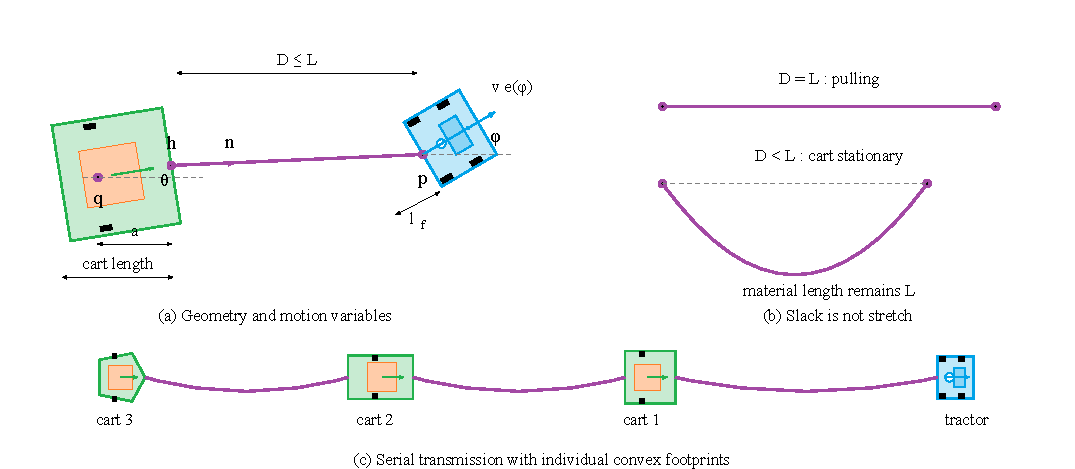
\includegraphics[width=\textwidth]{kinematics.pdf}
\caption{Vehicle geometry, slack--taut cable states, and serial transmission to passive carts.}
\label{fig:kinematics}
\end{figure*}
\subsection{Geometry and Operating Assumptions}
Let $\pp\in\mathbb R^2$ and $\phi$ denote the tractor rear-axle position and heading. The cable attaches at $\pp$ and at the cart hitch $\hh\in\mathbb R^2$. The cart heading is $\theta$, the hitch-to-axle offset is $a>0$, and $\ee(\alpha)=(\cos\alpha,\sin\alpha)^\top$. Its axle position is the algebraic output
\begin{equation}
\qq=\hh-a\ee(\theta).
\label{eq:axle}
\end{equation}
Define $\ee_\perp(\alpha)=[-\sin\alpha,\cos\alpha]^\top$ and
\begin{equation}
\begin{aligned}
D&=\|\pp-\hh\|_2,\\
\nn&=(\pp-\hh)/D,\\
D&>0,\\
D&\leq L.
\end{aligned}
\label{eq:cable}
\end{equation}
The cable material length $L$ is constant. The inequality $D<L$ describes slack accommodated by cable bending. The independent state is $\xx=(p_x,p_y,\phi,h_x,h_y,\theta)$.

The tractor follows bicycle kinematics with signed speed $v$, wheelbase $\ell_f$, steering angle $\delta$, and curvature $\kappa=\tan\delta/\ell_f$. The cart is assumed to stop immediately when no pulling motion is transmitted. In the pulling regime, a nominal hitch-mobility closure specifies that its hitch moves along the cable direction. With pulling speed $w\geq0$,
\begin{equation}\begin{aligned}
\dot\pp&=v\ee(\phi),\\
\dot\phi&=v\kappa,\\
\dot\hh&=w\nn,\\
\dot\theta&=\frac{w}{a}\nn^\top\ee_\perp(\theta).
\end{aligned}\label{eq:continuous}\end{equation}
This explicit first-order hitch-mobility closure specifies the pulling response. It implies
\begin{equation}
\dot\qq=w\bigl(\nn^\top\ee(\theta)\bigr)\ee(\theta),
\label{eq:nonholonomic}
\end{equation}
so the continuous axle velocity has no lateral component. The nonreversing cart rule is $w\nn^\top\ee(\theta)\geq0$. The tractor's $v$ can have either sign.

For $D<L$, the instantaneous unpulled state has $w=0$. On the taut boundary, outward tractor motion gives $w=\max\{0,\nn^\top\dot\pp\}$. Motion directed inward creates slack and stops the cart. The operating premise is quasistatic low-speed transport with sufficiently rapid stopping when pulling ceases. This first-order abstraction specifies the nominal motion used for planning; physical applicability depends on the stopping and hitch-mobility behavior of the cart.

\subsection{Euler Updates With an Inextensible Endpoint Closure}
For an interval of duration $\Delta t_k$, write $s_k=v_k\Delta t_k$ and $W_k=w_k\Delta t_k$. The optimization parameterizes motion by displacement increments and curvature. All independent states use first-order explicit Euler updates:
\begin{equation}\begin{aligned}
\pp_{k+1}&=\pp_k+s_k\ee(\phi_k),\\
\phi_{k+1}&=\phi_k+s_k\kappa_k,\\
\hh_{k+1}&=\hh_k+W_k\nn_k,\\
\theta_{k+1}&=\theta_k+\frac{W_k}{a}\nn_k^\top\ee_\perp(\theta_k).
\end{aligned}\label{eq:euler}\end{equation}
The axle position is evaluated algebraically from~\eqref{eq:axle} at every node.

The end-of-step cable condition closes $W_k$ algebraically. Set $c_k=\nn_k^\top\ee(\phi_k)$. From~\eqref{eq:euler},
\begin{equation}
\|\pp_{k+1}-\hh_{k+1}\|_2^2
=(D_k+s_kc_k-W_k)^2+s_k^2(1-c_k^2).
\label{eq:quadratic}
\end{equation}
Define the unconstrained closure displacement
\begin{equation}
\eta_k=D_k+s_kc_k-\sqrt{L^2-s_k^2(1-c_k^2)}.
\label{eq:eta}
\end{equation}
Then the common discrete mode relation is
\begin{equation}
W_k=\max\{0,\eta_k\}.
\label{eq:max}
\end{equation}

\begin{proposition}[Discrete unilateral closure]
Suppose $0<|s_k|<D_k\leq L$. Equation~\eqref{eq:max} is the minimum nonnegative hitch displacement along $\nn_k$ that satisfies the endpoint length bound. If the free endpoint remains within distance $L$ of the stationary hitch, $W_k=0$. Otherwise, the endpoint distance equals $L$ after the update. Moreover, $-L<\eta_k\leq |s_k|$.
\label{prop:closure}
\end{proposition}
\begin{IEEEproof}
The radicand in~\eqref{eq:eta} is positive. Since $D_k+s_kc_k>D_k-|s_k|>0$, the two roots of~\eqref{eq:quadratic} at squared distance $L^2$ delimit the feasible hitch-displacement interval. Its smaller endpoint is $\eta_k$, and its larger endpoint is positive. Intersecting this interval with $W_k\geq0$ gives the minimum $\max\{0,\eta_k\}$. Also, $D_k+s_kc_k>0$ and the square root is at most $L$, yielding $\eta_k>-L$. Let $r=|s_k|$ and $u=s_kc_k/r$. The function $ru-\sqrt{L^2-r^2+r^2u^2}$ increases on $[-1,1]$, since $\sqrt{L^2-r^2+r^2u^2}>|ru|$. Thus $\eta_k\leq D_k+r-L\leq r$.
\end{IEEEproof}

For $s_k=0$, the relation gives $W_k=0$ directly. The closure is exact for the stated discrete Euler model. Consequently,~\eqref{eq:euler}--\eqref{eq:max} preserve the endpoint bound in exact arithmetic and stop both hitch translation and cart rotation on an entirely slack step. A step crossing from slack to taut represents an average pulling increment over the integration interval. On the taut boundary, the first-order limit is $W_k/\Delta t_k\to\max\{0,\nn_k^\top\dot\pp_k\}$. The algebraic axle output has an $O(W_k^2)$ lateral displacement relative to its current heading, consistent with first-order state integration. Every compared method uses this Euler transcription with algebraic endpoint closure.

\subsection{Equivalent Exact Mode Representations}
Let $s_{\max}$ bound the signed tractor increment and let $D_{\min}$ bound the endpoint distance from below, with $0<s_{\max}<D_{\min}\leq L$. For fixed values of the geometric expression $\eta_k$, the graph of~\eqref{eq:max} has the exact complementarity representation
\begin{equation}
\begin{aligned}
 &W_k\geq0,\\
 &W_k-\eta_k\geq0,\\
 &W_k(W_k-\eta_k)=0.
\end{aligned}
\label{eq:comp}
\end{equation}
It also admits a binary representation with $z_k\in\{0,1\}$:
\begin{equation}\begin{aligned}
 &W_k\geq0,\\
 &W_k\geq\eta_k,\\
 &W_k\leq s_{\max}z_k,\\
 &W_k\leq\eta_k+L(1-z_k).
\end{aligned}\label{eq:minlp}\end{equation}
Proposition~\ref{prop:closure} establishes the sufficient constants $s_{\max}$ and $L$; an arbitrary large constant is unnecessary. For $z_k=0$,~\eqref{eq:minlp} forces $W_k=0$ and $\eta_k\leq0$. For $z_k=1$, it forces $W_k=\eta_k\geq0$. Conversely, either branch of~\eqref{eq:max} satisfies~\eqref{eq:minlp}. At $\eta_k=0$, either binary label describes the same state update. A conditional expression selecting $\eta_k$ when $\eta_k\geq0$ and zero otherwise is another implementation of the same graph. Fixing $z_k$ from an initial trajectory restricts this graph to the chosen mode sequence.

These equivalences concern the declared discrete model. They permit a controlled comparison of expression and solution strategies without changing the physical assumptions or discretization.

\subsection{Body Geometry, Collision Constraints, and Cable Routing}
Each body has a convex polygonal footprint of arbitrary shape. The local halfspace matrix and vector are computed from its actual vertices; no rectangular replacement is used. In local coordinates, let $\mathcal B=\{y:Gy\leq g\}$. Its world footprint is $\mathcal E_k=\RR(\alpha_k)\mathcal B+t_k$, where $\RR(\alpha)$ is the planar rotation matrix and $(t_k,\alpha_k)$ equals $(\pp_k,\phi_k)$ or $(\qq_k,\theta_k)$. For a convex obstacle $\mathcal O=\{y:Ay\leq b\}$, the OBCA distance certificate~\cite{obca2021} introduces $\lambda_k,\mu_k\geq0$ for a prescribed planning clearance $d_{\rm plan}>0$, satisfying
\begin{equation}\begin{aligned}
 &G^\top\mu_k+\RR(\alpha_k)^\top A^\top\lambda_k=0,\\
 &\|A^\top\lambda_k\|_2\leq1,\\
 &(At_k-b)^\top\lambda_k-g^\top\mu_k\geq d_{\rm plan}.
\end{aligned}\label{eq:obca}\end{equation}
The same dual construction is imposed between the two vehicle bodies and against workspace walls. Independent polygon-distance evaluation subsequently checks the primal trajectory rather than relying on the dual variables or solver status alone.

Cable collision is treated separately from body separation. For $D<L$, the routing audit constructs the smooth planar curve
\begin{equation}
\mathbf r(t)=\hh+t(\pp-\hh)+4\alpha t(1-t)\nn_\perp,
\label{eq:route}
\end{equation}
for $t\in[0,1]$, where $\nn_\perp=(-n_y,n_x)^\top$ and the lateral bow amplitude $\alpha\geq0$ is selected so that the analytic arc length equals $L$. Its arc length is
\begin{equation}
\mathcal L(\alpha)=\tfrac12\sqrt{D^2+16\alpha^2}
+\frac{D^2}{8\alpha}\operatorname{asinh}(4\alpha/D).
\label{eq:arclength}
\end{equation}
The continuous limit at zero amplitude is $D$. Either lateral orientation may be checked; a taut cable is a straight segment. In the most compact mechanism cases, a symmetric curve can enter a vehicle near an attachment. The audit then also tests the smooth asymmetric family obtained by replacing $4t(1-t)$ with $f_\beta(t)=4t(1-t)[1+\beta(2t-1)]$. Its amplitude is selected from $\int_0^1\sqrt{D^2+\alpha^2[f_\beta' (t)]^2}\,dt=L$, checked by independent numerical quadrature. This routing freedom changes neither endpoint kinematics nor material length. The warehouse solver comparisons use the same symmetric routing filter throughout; asymmetric routes are an additional geometric witness for the compact mechanism suite. A segmented evaluation of the curve tests walls, obstacles, and body interiors, with the quadratic chord-error bound applied to obstacle checks. An accepted curve is a per-node geometric routing witness: it establishes the existence of a collision-free cable route of the prescribed length at that configuration. Continuous shape evolution and snag-free execution require a physical cable-interaction model. All methods use this same routing filter.

\subsection{Serial Cable-Towed Carts}
For cart $i$, let $\hh_i$ be its front hitch, $\theta_i$ its heading, $a_i$ its hitch-to-axle distance, and $b_i$ the distance from the axle to the rear attachment. Its rear attachment is $\mathbf t_i=\hh_i-(a_i+b_i)\ee(\theta_i)$. Cable $i$ connects $\hh_i$ to $\mathbf t_{i-1}$, with $\mathbf t_0=\pp$. Define the material length $L_i$, endpoint distance $D_i=\|\mathbf t_{i-1}-\hh_i\|_2$, and direction $\nn_i=(\mathbf t_{i-1}-\hh_i)/D_i$. Once the upstream attachment displacement $\Delta\mathbf t_{i-1}$ is known, the same endpoint closure gives
\begin{equation}\begin{aligned}
c_i&=\nn_i^\top\Delta\mathbf t_{i-1},\\
W_i&=\max\!\left\{0,D_i+c_i-\sqrt{L_i^2-\|\Delta\mathbf t_{i-1}\|^2+c_i^2}\right\}.
\end{aligned}\label{eq:serial}\end{equation}
The hitch and heading use the Euler updates in~\eqref{eq:euler} with indices $i$. Propagation proceeds from the tractor toward the final cart. A stationary upstream attachment produces zero downstream displacement, consistent with the stop-on-slack rule. Positive radicands and step bounds are required at every link. The OBCA construction extends to all body pairs and all body--obstacle pairs, using each cart's own footprint.

\subsection{Optimization Problem}
For a common grid of $N$ intervals, the decision variables are the states, $(s_k,\kappa_k,W_k)$, and OBCA dual variables, with binary variables only in~\eqref{eq:minlp}. The objective is
\begin{equation}
\begin{aligned}
J&=\sum_{k=0}^{N-1}\ell_k+\gamma\sum_{k=1}^{N-1}(\kappa_k-\kappa_{k-1})^2,\\
\ell_k&\geq s_k,\\
\ell_k&\geq -s_k.
\end{aligned}
\label{eq:cost}
\end{equation}
The first term measures tractor travel; the second discourages abrupt changes in the curvature sequence. The nonnegative travel epigraph $\ell_k$ equals $\max\{s_k,-s_k\}$ at a minimum. Reported costs are recomputed from the actual controls with this exact travel value. The same weight $\gamma$ is used by every method, with its numerical value listed in the experimental settings.

The constraints are the prescribed initial state,~\eqref{eq:euler}, one exact mode representation,~\eqref{eq:obca}, the terminal transport task, and
\begin{equation}\begin{aligned}
 &s_k\geq-s_{\max},\\
 &s_k\leq s_{\max},\\
 &\kappa_k\geq-R_{\min}^{-1},\\
 &\kappa_k\leq R_{\min}^{-1},\\
 &D_k\geq D_{\min},\\
 &D_k\leq L,\\
 &W_k\nn_k^\top\ee(\theta_k)\geq0.
\end{aligned}\label{eq:bounds}\end{equation}
The stated relation among $s_{\max}$, $D_{\min}$, and $L$ satisfies Proposition~\ref{prop:closure}. The terminal task specifies a rear-axle goal region and desired tractor and cart headings. This permits side loading, turns, and return routes. The numerical implementation bounds headings in $[-\pi,\pi]$ and positions within the workspace; task headings are represented continuously within that interval. All methods use identical state and terminal bounds for each case. Numerical dimensions, tolerances, and solver settings are collected in Section~V.

\subsection{A Reachability Separation From Rigid Coupling}
Consider a conventional rigid-drawbar system with the same vehicle bodies and drawbar length $L$. Its hitch relation is
\begin{equation}
\pp=\qq+(a+L)\ee(\theta).
\label{eq:rigid}
\end{equation}
The tongue is fixed relative to the cart and pivots at the tractor attachment. Both vehicles may move forward or backward. This comparator has the same fully extended longitudinal span as the initially taut cable system.

For this comparison, both footprints are rectangles. Let $b_r$ be the cart rear overhang, $c_f$ the tractor's forward extent, and $w_r,w_f$ the respective half-widths. Define $A_0=a+L+b_r$. The vehicles start aligned with the horizontal direction inside an infinite vertical strip. After subtracting wall clearances, the available horizontal width is $A_0+c_f+\epsilon$.

\begin{theorem}[Rigid strip barrier]
If
\begin{equation}
\begin{aligned}
 &\epsilon>0,\\
 &\epsilon<B_*,\\
 &B_*=\min\{B_\theta,B_\phi\},\\
 &B_\theta=\sqrt{A_0^2+w_r^2}-A_0,\\
 &B_\phi=\sqrt{c_f^2+w_f^2}-c_f.
\end{aligned}
\label{eq:barrier}
\end{equation}
no continuous collision-free configuration path satisfying~\eqref{eq:rigid} can reorient the initially aligned combination to cart heading $\pi/2$, regardless of the sequence of forward and backward controls.
\label{thm:rigid}
\end{theorem}
\begin{IEEEproof}
Define the limiting cart and tractor headings by $\theta_*=\arctan(w_r/A_0)$ and $\phi_*=\arctan(w_f/c_f)$, respectively. Within the angle box $|\theta|\leq\theta_*$, $|\phi|\leq\phi_*$, the horizontal distance from the cart's leftmost corner to the tractor's rightmost corner is
\begin{equation}
H=A_0\cos\theta+w_r|\sin\theta|
+c_f\cos\phi+w_f|\sin\phi|.
\label{eq:span}
\end{equation}
It is a lower bound on the occupied width, independent of translation. Each of the two angle-dependent terms is at least its initial value, $A_0$ or $c_f$, within this box. Any continuous path from zero headings to the target must first reach the box boundary. There, at least one term reaches its maximum, either $\sqrt{A_0^2+w_r^2}$ or $\sqrt{c_f^2+w_f^2}$. Thus $H\geq A_0+c_f+B_*>A_0+c_f+\epsilon$, contradicting the available width. The proof imposes no restriction on control direction.
\end{IEEEproof}

Cable coupling allows the taut cable direction to differ from the cart heading. Slack further permits the tractor to reverse and rotate while the cart waits, then pull it into the vertical transport direction. Section~V constructs numerical trajectories for a parameterized family satisfying~\eqref{eq:barrier}. Theorem~\ref{thm:rigid} certifies the rigid system's continuous geometric obstruction, while independent Euler replay and per-node cable-route checks establish feasibility of the cable maneuvers under the prescribed discrete model.
\section{Optimization-Based Motion Planning}
The optimization-based planner refines a feasible seed through relaxed initialization, feasible control restoration, and direct-max optimization. Replay-derived clearance reserves guide refinement in the presence of integration drift. Independent replay determines acceptance of optimized and recovered trajectories.

\subsection{Common Initialization and Relaxed Refinement}
For each task, a tractor control sequence is constructed and validated before optimization. Its causal rollout supplies the common states and cable-mode sequence. Every strategy receives the same mesh, geometry, continuous initial values, and OBCA dual initialization. Initial dual multipliers represent polygon support directions using nonnegative local halfspace multipliers; the optimizer subsequently changes them freely.

The first stage replaces only the product equality in~\eqref{eq:comp} by
\begin{equation}\begin{aligned}
 &W_k\geq0,\\
 &W_k\geq\eta_k,\\
 &W_k(W_k-\eta_k)\leq\varepsilon_c.
\end{aligned}\label{eq:relax}\end{equation}
The objective and geometric constraints are retained. This stage allows the initializer to move between switching schedules. Its controls are propagated causally from the initial state using~\eqref{eq:euler}--\eqref{eq:max}. The rollout restores the discrete cable relation, although obstacle clearance or terminal conditions can change. Before the next solve, control restoration searches toward the common feasible seed. It accepts a new initializer only when the complete physical validator passes and the original-grid clearance is at least $d_{\rm plan}$. Otherwise, the common seed initializes refinement. A physically validated anchor remains available throughout the pipeline.

\subsection{Replay-Guided Clearance Reserves}
Let $\bar\xx_k$ be the causal rollout on the optimization grid and $\widetilde\xx_k$ its finer Euler replay sampled at the same control boundaries. For local vertex $v_{b,j}$ of body $b$, let $V_{b,j}(\xx)$ denote its world position. Define
\begin{equation}
r_{k,b}=\max_j\|V_{b,j}(\bar\xx_k)-V_{b,j}(\widetilde\xx_k)\|_2.
\label{eq:reserve}
\end{equation}
The corresponding convex combinations of vertices differ by at most $r_{k,b}$, so this quantity bounds the Hausdorff deviation of the two sampled polygons. Their distances to a fixed obstacle differ by at most the same amount; a two-body distance can change by the sum of the two reserves.

The direct-max refinement uses $d_{\rm plan}+r_{k,b}$ against obstacles and walls, and $d_{\rm plan}+r_{k,1}+r_{k,2}$ between bodies. The reserves are fixed during the solve and change only the internal OBCA clearance requirements. Physical geometry and final required clearance remain unchanged. The initializer remains physically validated, although the additional reserves and initialized dual multipliers need not form a feasible point of the buffered nonlinear program.

These measured deviations describe the initializer, and optimization can move away from it. Every result therefore undergoes the same independent validation. The proposed planner uses the measured reserves directly. Section~V isolates their effect by comparison with zero reserves and reserves capped by available clearance.

The maximum is implemented directly, without smoothing. AMPL supplies the active-branch derivatives away from switching points to Ipopt. Actual feasibility is evaluated from the returned trajectory, including outputs produced at iteration or time limits.

\subsection{Control Recovery and Terminal Restoration}
Control recovery extracts useful route improvements from candidates that fail independent acceptance. It operates on signed tractor increments and yaw increments, $y_k=s_k\kappa_k$, and reconstructs every state causally to enforce the discrete kinematics.

Let $(s^a,y^a)$ belong to the lowest-cost validated anchor available and $(s^c,y^c)$ to a candidate. A decreasing sequence of weights $\alpha\in(0,1]$ generates
\begin{equation}\begin{aligned}
 s_k(\alpha)&=(1-\alpha)s_k^a+\alpha s_k^c,\\
 y_k(\alpha)&=(1-\alpha)y_k^a+\alpha y_k^c.
\end{aligned}\label{eq:blend}\end{equation}
Interpolating signed increments can change their signs, so yaw interpolation alone does not preserve curvature bounds. A scalar shift followed by clipping enforces the per-step yaw limits and the required terminal tractor heading. With $u_k=|s_k|/R_{\min}$ and positive weights $\omega_k$, the projection uses
\begin{equation}\begin{aligned}
 \widehat y_k&=\min\{u_k,\max\{-u_k,y_k+\lambda\omega_k\}\},\\
 \sum_k\widehat y_k&=\phi_{\rm goal}-\phi_0.
\end{aligned}\label{eq:yawprojection}\end{equation}
The sum is monotone in $\lambda$, permitting bisection. If its target lies outside the attainable interval, the trial is skipped. Curvature is recovered as $\widehat y_k/s_k$ for nonzero increments and set to zero for a zero increment. Projection is applied to the candidate and again after interpolation.

Control interpolation also changes the cart endpoint. A three-parameter shooting correction uses a fixed terminal window to restore its cart axle position and heading. One basis distributes a signed-travel adjustment along that window; two zero-sum yaw bases apply opposing pulses to adjacent thirds. Their zero sums preserve terminal tractor heading. A finite-difference Newton step with line search reduces the three cart endpoint residuals, subject to the original travel and curvature bounds. The window does not depend on the optimizer returning an exactly straight terminal segment. This correction changes controls only; all states and cable modes are recomputed using the same closure.

Each trial is checked before terminal correction, so a valid causal rollout is preserved without unnecessary shooting. The exact-refinement candidate is processed before earlier candidates. Every recovered trial must reduce the anchor objective and pass the complete common validator. The first accepted weight for each candidate is retained, and the lowest-cost result is returned. Initial restoration additionally requires the planning clearance and uses a short, conservative weight sequence. Final recovery explores the full sequence. If either allowance is exhausted, the validated anchor remains available. Algorithm~\ref{alg:planner} shows the nested structure.

\begin{algorithm}[!t]
\caption{Trajectory refinement with validated control recovery}
\label{alg:planner}
\DontPrintSemicolon\SetAlgoVlined
\SetKwInput{KwIn}{Input}\SetKwInput{KwOut}{Output}
\KwIn{Geometry, task, validated seed $S_0$, nominal allowance $T$}
\KwOut{Lowest-cost independently validated trajectory}
Start elapsed-time clock; $A\gets S_0$\;
$S_r\gets$ relaxed solve using~\eqref{eq:relax}\;
$S_e\gets$ validated control restoration toward $S_0$, or $S_0$\;
Compute finer replay and reserves~\eqref{eq:reserve}\;
$S_*\gets$ direct-max refinement, reserving recovery time\;
\ForEach{candidate $S$ in $\{S_r,S_e,S_*\}$}{
 \If{$S$ passes validation and $J(S)<J(A)$}{$A\gets S$\;}
}
\ForEach{available candidate $S$ in $\{S_*,S_e,S_r\}$}{
 \ForEach{decreasing recovery weight $\alpha$}{
  \If{the remaining budget is exhausted}{stop recovery\;}
  Blend and project controls using~\eqref{eq:blend}--\eqref{eq:yawprojection}\;
  $S_\alpha\gets$ causal rollout of the projected controls\;
  \If{$S_\alpha$ fails validation}{Apply terminal-window correction; roll out again\;}
  \If{$J(S_\alpha)<J(A)$ and $S_\alpha$ passes validation}{
   Retain $S_\alpha$; advance to the next candidate\;
  }
 }
}
\Return lowest-cost member of $\{A,\text{retained recovery trials}\}$\;
\end{algorithm}

\subsection{Independent Acceptance and Computational Accounting}
Candidates are recursively replayed from the prescribed initial state without resetting to optimized nodes. The checks cover state consistency, control and grid-state bounds, initial-pose clearance, unilateral cable closure, the nonreversing cart rule, terminal conditions, body clearance, and a geometric cable route at the original-grid nodes. A second replay subdivides every interval using the same Euler rule and checks body clearance and the transport endpoint. Polygon distances are computed directly from primal geometry, independently of the OBCA multipliers. Finer replay assesses grid sensitivity; cable routing remains the per-node witness described in Section~III.

We distinguish a newly validated planner output from retention of the common initial trajectory. Outputs from numerical optimization and control recovery are also reported separately. The retained objective can never exceed that of a valid common seed. Total backend time includes data preparation, process startup, all optimization and recovery stages, and validation. A final in-progress check can exceed the nominal allowance; reported wall-clock time includes that excess.

\subsection{Comparison Methods and Matched Ablations}
The comparisons cover three numerical choices. First, \emph{MAX}, \emph{LOGIC}, \emph{COMP}, and \emph{MINLP} implement the same cable graph using a direct maximum, a conditional expression, exact complementarity, and binary constraints, respectively. MAX is the direct formulation baseline of this paper. The proposed method also uses that maximum in its refinement and rollout. MINLP uses BONMIN branch-and-bound with Ipopt and the HSL sparse linear solver MA57 for nonlinear subproblems; the nonconvex solves provide no general global-optimality certificate.

Second, \emph{FIX}, inspired by the mode-sequence strategy of~\cite{zhang2026}, holds the cable-mode sequence extracted from the common initial trajectory fixed. \emph{PORT}, adapted from the alternative-mode idea of~\cite{yang2022}, evaluates the initial schedule and two schedules with locally shifted switching labels. The source considers simultaneous modes of several cables over a prediction window; this single-cable adaptation enumerates temporal schedules. Duplicate schedules are removed before the remaining sequential branches share one total allowance and common continuous initialization. If the initial schedule has no switching event, this adaptation reduces to FIX.

Third, a factorial comparison crosses initial restoration (on/off) with reserve setting (zero/measured/capped). Comparing rows that differ in one setting isolates that factor under a common overall allowance. A paired \emph{No final recovery} result uses the exact outputs recorded before final recovery in the proposed run, retaining initial restoration. A paired \emph{No terminal correction} replay removes only shooting from final recovery. \emph{MAX+recovery} applies the same final recovery mechanism to direct MAX. The first-stage output supplies a relaxed-only comparison.

\emph{Replay-guided refinement (RGR)} combines relaxed initialization, causal rollout, and measured reserves, allocating the remaining allowance to direct refinement. \emph{Relaxed rollout planning (RRP)} removes only the reserves from RGR. These two strategies isolate reserve guidance in a solve-only workflow. The factorial and paired comparisons isolate the components of the complete proposed method. Numerical settings are specified with the experiments.

\section{Simulation Experiments}
The evaluation separates the mechanical value of cable coupling from numerical planning performance. A parameterized strip family tests reachability; nine square warehouse tasks compare algorithms. Matched ablations, footprint variations, and a serial formation examine the contributing mechanisms and extensions.

\subsection{Unified Settings and Constructively Feasible Maps}
The implementation uses MATLAB R2024a, AMPL, Ipopt 3.12.13, BONMIN 1.8.9, and HSL MA57 on a Windows workstation with an Intel Core i9-12900 processor. MATLAB uses one computation thread, and optimization jobs run sequentially. All state updates and replay checks use first-order explicit Euler. Table~\ref{tab:settings} specifies the common geometry, tolerances, and computational settings.

\begin{table}[!t]
\centering\caption{Shared geometry, numerical settings, and validation thresholds}
\label{tab:settings}\footnotesize
\setlength{\tabcolsep}{4pt}
\begin{tabular}{ll}
\toprule
Quantity & Value\\
\midrule
Workspace & $16\times16$ m\\
Tractor footprint; wheelbase & $0.60\times0.70$ m; $0.40$ m\\
Nominal cart footprint & $1.05\times1.10$ m\\
Hitch-to-axle / rear overhang & $0.70/0.35$ m\\
Material cable length & $1.335$ m\\
Minimum turning radius & $0.40$ m\\
Endpoint lower bound / step bound & $0.25/0.18$ m\\
Heading bounds & $[-\pi,\pi]$ rad\\
Required / planning clearance & $0.10/0.12$ m\\
Curvature regularization $\gamma$ & $0.002$\\
Original-grid cart position bound & $0.12$ m per coordinate\\
Original-grid cart heading bound & $0.008$ rad\\
Tractor terminal heading bound & $10^{-5}$ rad\\
Finer Euler replay subdivisions & $8$ per interval\\
Fine cart position / heading bounds & $0.27$ m per coordinate / $0.025$ rad\\
Common computation allowance & $30$ s\\
Direct NLP iteration ceiling & $3000$\\
Relaxed stage allowance / iterations & $5$ s / $300$\\
Relaxation product bound & $10^{-4}$ m$^2$\\
Refinement iteration ceiling & $600$\\
Initial restoration / final reserve & $4/4$ s\\
Initial restoration weights & $1/8,1/32,1/128,1/512,1/1024$\\
Final recovery weights & $1,1/2,\ldots,1/1024$\\
Yaw projection bisections & $65$\\
Terminal correction iterations & At most $5$\\
Terminal correction window & $\min\{N,\max\{9,\lceil N/4\rceil\}\}$\\
PORT unique schedules / allowance & At most $3$ / $30$ s\\
\bottomrule
\end{tabular}
\end{table}

The tractor polygon is referenced to its rear axle and extends forward. The cart polygon extends to either side of its axle; its front hitch lies at the forward center. The cable joins the tractor rear axle to that hitch, as defined in Fig.~\ref{fig:kinematics}. Complete vertices, maps, controls, source code, solver inputs, logs, and validation records are available in the reproducibility package at \url{https://anonymous.4open.science/r/Cable-Towing-Trailer-361F/}. Its README maps each comparison to the source files and records, with file hashes for integrity checks.

The nine layouts are defined by modular rack rows, picking aisles, cross aisles, pallet staging areas, and packing stations before trajectory construction. Their common outer boundary is $16\times16$ m. W01--W09 respectively represent a blocked-aisle transfer, a two-aisle rack-end transfer, a cross-aisle exchange, an adjacent-aisle return, two successive offsets between storage blocks, a packing-area turn, a pallet-staging bypass, a return between mixed rack orientations, and a perimeter replenishment circuit. The nominal picking aisles in W01--W08 are $1.7$ m wide for a $1.1$ m cart; cross aisles provide the space needed for the complete formation to turn. Discrete racks leave connected access routes and functional work areas.

Feasible control sequences are constructed within the fixed layouts and checked by the common validator. All comparisons use the same nine maps, accepted seeds, model parameters, and physical acceptance criteria. A single configuration of the proposed method is applied across this designed benchmark.

\begin{table}[!t]
\centering\caption{Warehouse layouts, meshes, and minimum replayed body clearances}
\label{tab:cases}
\footnotesize\begin{tabular}{lrrrr}
\toprule
Case & $N$ & Objects & Seed (m) & Proposed (m)\\
\midrule
W01 & 98 & 11 & 0.126 & 0.113\\
W02 & 135 & 8 & 0.196 & 0.168\\
W03 & 100 & 11 & 0.137 & 0.126\\
W04 & 142 & 12 & 0.170 & 0.159\\
W05 & 100 & 12 & 0.103 & 0.122\\
W06 & 91 & 12 & 0.162 & 0.119\\
W07 & 106 & 11 & 0.111 & 0.127\\
W08 & 127 & 12 & 0.197 & 0.182\\
W09 & 300 & 12 & 0.142 & 0.207\\
\bottomrule\end{tabular}
\end{table}

Table~\ref{tab:cases} reports the map obstacles, mesh sizes, and minimum body clearances under finer replay for the common initial trajectories and final proposed outputs. Figure~\ref{fig:nine-cases} uses identical physical map dimensions, canvas sizes, and vehicle scale. Cyan and green denote the tractor and cart; orange racks, yellow pallets, and violet packing stations identify distinct warehouse objects. Faint footprints show swept body positions. S and G mark the starting and final tractor configurations. Statistics include all nine layouts.

\begin{figure*}[!t]
\centering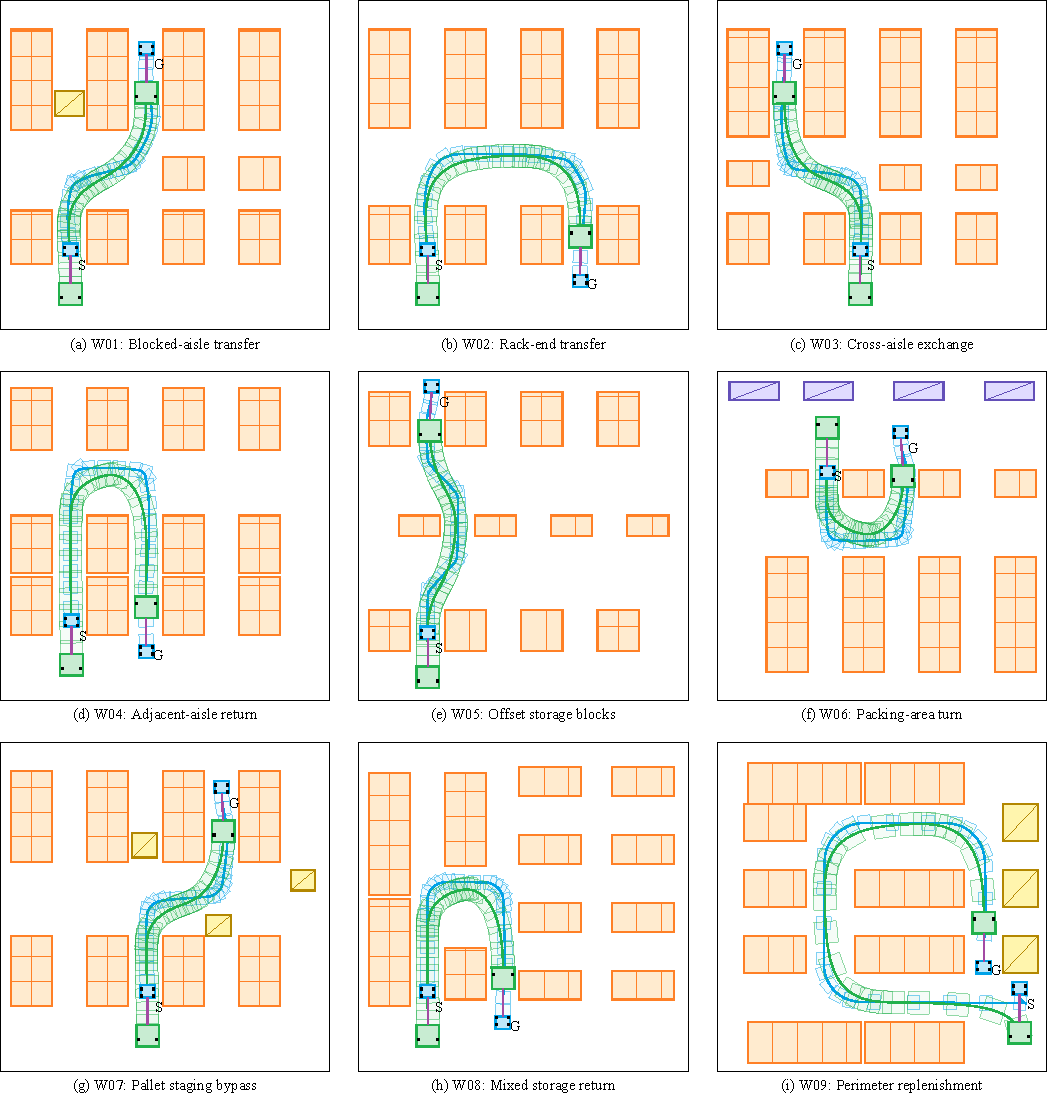
\includegraphics[width=\textwidth]{warehouse_cases.pdf}
\caption{Nine distinct confined warehouse tasks with identical workspace dimensions and vehicle scale.}
\label{fig:nine-cases}
\end{figure*}

All cable strategies receive the same feasible control seed, mesh, goal, physical clearance, and dual initialization for each map. Method order rotates across cases. The study measures trajectory improvement from constructive feasible initializations. The nominal allowance allocates optimization-stage time; reported elapsed time also includes pipeline overhead. Measured backend time includes serialization, startup, validation, and termination overhead. Time-limited outputs can be accepted if they pass all independent checks.

The transport tasks terminate in arrival regions around the prescribed cart pose. Both endpoint tests use that same goal: original-grid position and heading bounds are $0.12$ m per coordinate and $0.008$ rad; finer Euler replay uses $0.27$ m and $0.025$ rad. Across the nine proposed outputs, the actual finer-replay Euclidean position errors range from $0.050$ to $0.155$ m, and the maximum cart heading error is $0.02197$ rad ($1.26^\circ$). The maximum original-grid Euclidean error is $0.1375$ m. Per-case errors are supplied with the numerical records. Required body clearance remains $0.10$ m at both resolutions. These endpoint conditions define warehouse transfer arrival; precision docking and tracking are subsequent control tasks.

\subsection{Mechanical Benefit Relative to a Rigid Drawbar}
The strip study varies cable length over $1.3$, $1.5$, and $1.7$ m, tractor turning radius over $0.4$ and $0.5$ m, and excess strip width over $0.30$, $0.60$, and $0.85$ times the barrier in~\eqref{eq:barrier}. The resulting 18 tasks satisfy Theorem~\ref{thm:rigid}. The rigid comparator uses the same body dimensions, fully extended initial span, clearance, and target heading, and may reverse. Its reorientation is excluded by the geometric barrier.

All 18 cable trajectories pass independent Euler replay and fixed-material-length cable-route checks. Figure~\ref{fig:mechanism} shows the mechanism: the tractor reverses and rotates while the cart waits, then resumes pulling. Endpoint separation decreases during repositioning without changing material length. Three compact cases require the asymmetric cable-route family, using shape parameters $\beta\in\{0,\pm0.25,\pm0.50,\pm0.75\}$ and a material-length residual below $10^{-7}$ m. The original-grid and finer-replay node configurations are checked; the vehicle trajectories are unchanged.

\begin{figure*}[!t]
\centering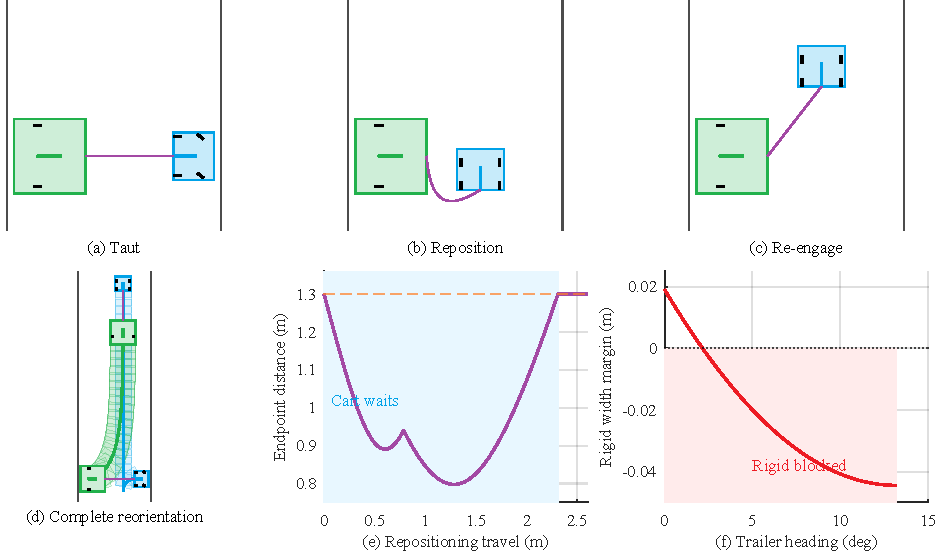
\includegraphics[width=\textwidth]{mechanism_revision.pdf}
\caption{Slack-enabled reorientation and the geometric obstruction imposed by an equal-length rigid drawbar.}
\label{fig:mechanism}
\end{figure*}

On the nine warehouse layouts, direct transcription with the rigid drawbar returns 0/9 new validated trajectories under the common allowance, compared with 8/9 for cable MAX. Both use the same footprints, taut connection length, task configurations, mesh, and direct nonlinear-solve strategy. Their shared initial controls are replayed through their respective kinematics; the resulting rigid rollout need not be feasible. The rigid cart may reverse. These attempts report numerical outcomes from that initialization, whereas Theorem~\ref{thm:rigid} independently establishes mechanical impossibility for the strip family. The controlled cable-algorithm comparison uses feasible initial trajectories for every method.


\subsection{Controlled Numerical Comparisons}
The comparisons evaluate feasible-seed trajectory refinement under the common discrete model. MAX, LOGIC, COMP, and MINLP compare representations of the same discrete cable relation. FIX and PORT compare mode strategies adapted from~\cite{zhang2026,yang2022}. After duplicate removal, PORT has one schedule on W01--W08 and three on W09; its single-schedule cases reduce to FIX, with separate time-limited runs. RGR uses replay reserves after causal rollout; the proposed method first restores a feasible initializer and includes final control recovery. Retained costs are recomputed from accepted controls. Mean travel reduction averages each case's reduction relative to its own common seed.

\begin{table*}[!t]
\centering\caption{Common-allowance comparison on nine warehouse tasks}
\label{tab:main}
\footnotesize\begin{tabular}{lrrrrrrr}
\toprule
Method & New & NLP & $\Delta J\geq1\%$ & $\Delta J$ (\%) & $\Delta l$ (\%) & $t_{50}$ (s) & $t_{90}$ (s)\\
\midrule
Proposed & 9/9 & 7/9 & 9/9 & 4.44 & 4.36 & 31.03 & 31.76\\
MAX & 8/9 & 8/9 & 6/9 & 1.02 & 0.97 & 30.97 & 33.91\\
LOGIC & 2/9 & 2/9 & 2/9 & 1.09 & 1.07 & 30.72 & 35.10\\
COMP & 2/9 & 2/9 & 2/9 & 0.91 & 0.91 & 30.68 & 32.32\\
FIX & 2/9 & 2/9 & 2/9 & 0.71 & 0.70 & 30.73 & 32.26\\
PORT & 3/9 & 3/9 & 2/9 & 0.78 & 0.77 & 31.12 & 34.03\\
MINLP & 0/9 & 0/9 & 0/9 & 0.00 & 0.00 & 31.41 & 32.10\\
RGR & 7/9 & 7/9 & 5/9 & 3.04 & 2.92 & 33.01 & 36.53\\
\bottomrule\end{tabular}
\end{table*}

Table~\ref{tab:main} distinguishes new validated planner outputs (New) from validated nonlinear-solver outputs before recovery (NLP); both counts have denominator nine. Every method retains a validated trajectory because the common feasible seed remains available. The proposed method produces 9/9 new outputs, including 7/9 accepted directly from its nonlinear solves, and improves the objective in all nine tasks. Its mean per-case travel reduction is 4.36\%, compared with 0.97\% for MAX; median backend times are 31.03 and 30.97 s. Its retained objective is lower than MAX in eight cases and lowest among the eight methods in four. MAX gives the lower objective on W09. The proposed method is faster than MAX in six cases, with comparable median time overall.
The objective reduction reaches at least one percent in 9/9 cases for Proposed and 6/9 for MAX. The statistics $t_{50}$ and $t_{90}$ denote median and 90th-percentile backend times. Together, these results support a quality and new-output acceptance advantage within the common computational allowance.


\begin{figure*}[!t]
\centering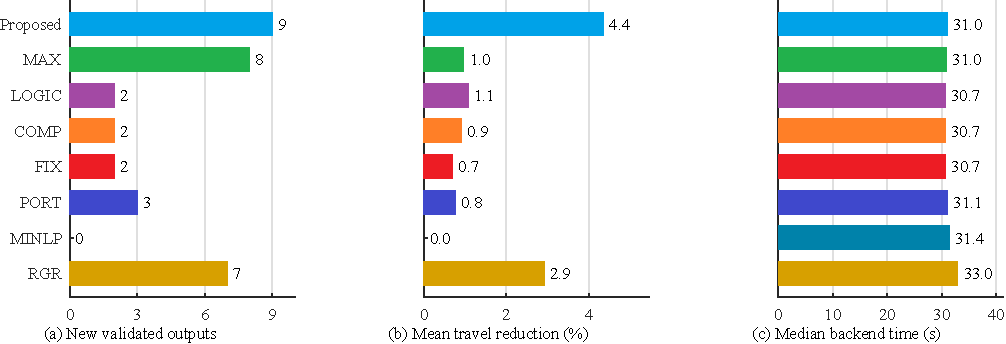
\includegraphics[width=.98\textwidth]{comparison_summary.pdf}
\caption{New validated trajectories, mean travel reduction, and measured backend time across all nine tasks.}
\label{fig:comparison}
\end{figure*}

\begin{table*}[!t]
\centering\caption{Retained objectives; asterisks mark no improvement over the common seed}
\label{tab:per-case}
\footnotesize\begin{tabular}{lrrrrrrrr}
\toprule
Case & Proposed & MAX & LOGIC & COMP & FIX & PORT & MINLP & RGR\\
\midrule
W01 & 12.12 & 13.15 & 13.29$^*$ & 13.29$^*$ & 13.29$^*$ & 13.29$^*$ & 13.29$^*$ & 12.83\\
W02 & 16.99 & 18.80 & 17.66 & 19.01$^*$ & 18.31 & 18.31 & 19.01$^*$ & 19.01$^*$\\
W03 & 12.47 & 13.09 & 13.23$^*$ & 13.23$^*$ & 13.23$^*$ & 13.23$^*$ & 13.23$^*$ & 12.13\\
W04 & 19.41 & 20.13 & 19.66 & 20.21$^*$ & 19.66 & 19.66 & 20.21$^*$ & 20.17\\
W05 & 13.09 & 13.13 & 13.33$^*$ & 13.33$^*$ & 13.33$^*$ & 13.33$^*$ & 13.33$^*$ & 12.78\\
W06 & 11.86 & 12.28$^*$ & 12.28$^*$ & 12.28$^*$ & 12.28$^*$ & 12.28$^*$ & 12.28$^*$ & 12.28$^*$\\
W07 & 12.80 & 12.98 & 13.07$^*$ & 13.07$^*$ & 13.07$^*$ & 13.07$^*$ & 13.07$^*$ & 12.25\\
W08 & 15.05 & 15.20 & 15.44$^*$ & 14.41 & 15.44$^*$ & 15.44$^*$ & 15.44$^*$ & 15.44$^*$\\
W09 & 31.23 & 30.98 & 31.60$^*$ & 31.11 & 31.60$^*$ & 31.41 & 31.60$^*$ & 30.01\\
\bottomrule\end{tabular}
\end{table*}

Figure~\ref{fig:details} compares the proposed and MAX tractor paths on the predeclared rack-end, double-offset, and perimeter tasks. Each panel includes the actual vehicle outlines and swept footprints. A route that shortens the tractor path is useful only if the passive cart and cable also satisfy validation. Figure~\ref{fig:modes} plots the perimeter task's initial repositioning phase against accumulated tractor travel. The transmitted cart displacement stays zero on slack steps while the tractor can move backward and change heading.

\begin{figure*}[!t]
\centering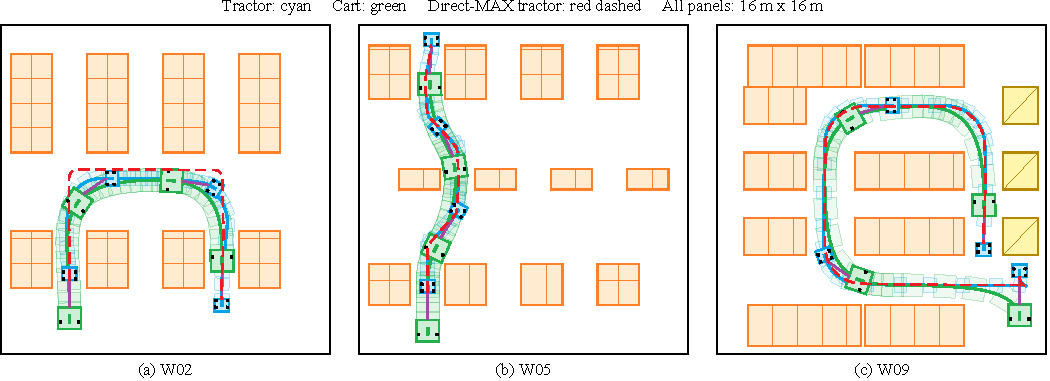
\includegraphics[width=.98\textwidth]{trajectory_details.pdf}
\caption{Validated paths and swept body footprints on three representative square warehouse tasks.}
\label{fig:details}
\end{figure*}

\subsection{Component Ablations and Repeated Runs}
The ablations test how individual stages contribute to accepted trajectory quality under fixed physical thresholds. Causal control restoration enforces consistency between controls and states, initial restoration supplies a validated refinement anchor, and replay reserves guide clearance during optimization. The paired recovery tests reuse identical preceding outputs, while the factorial study varies initial restoration and reserve treatment one factor at a time.

\begin{table*}[!t]
\centering\caption{Control-recovery ablations and solve-only strategy comparisons}
\label{tab:ablation}
\footnotesize\begin{tabular}{lrrrr}
\toprule
Variant & New & Impr. & $\Delta l$ (\%) & $t_{50}$ (s)\\
\midrule
Proposed & 9/9 & 9/9 & 4.36 & 31.03\\
No final recovery (paired) & 9/9 & 9/9 & 2.68 & 27.91\\
No terminal correction (paired) & 9/9 & 9/9 & 3.18 & --\\
RGR & 7/9 & 6/9 & 2.92 & 33.01\\
No reserves (RRP) & 0/9 & 0/9 & 0.00 & 31.78\\
MAX + recovery & 9/9 & 9/9 & 1.07 & 24.90\\
Relaxed stage only & 0/9 & 0/9 & 0.00 & --\\
\bottomrule\end{tabular}
\end{table*}

Both Proposed and MAX+recovery produce 9/9 new validated outputs. Their mean travel reductions are 4.36\% and 1.07\%, respectively, showing the quality benefit of the complete refinement workflow beyond adding recovery to MAX. Final recovery supplies four of the nine proposed outputs and raises mean reduction from 2.68\% at the identical paired prefix to 4.36\%. Removing terminal correction gives 3.18\%. The no-terminal-correction row reuses that same prefix, so a separate complete-pipeline runtime is inapplicable. The relaxed-only row reports first-stage acceptance and quality.

\begin{table*}[!t]
\centering\caption{Factorial comparison of initial restoration and three reserve settings}
\label{tab:factorial}
\footnotesize\begin{tabular}{lllrrrr}
\toprule
Variant & Initial restoration & Reserves & New & $\Delta J$ (\%) & $\Delta l$ (\%) & $t_{50}$ (s)\\
\midrule
F1 & On & Capped & 9/9 & 4.19 & 4.12 & 30.82\\
F2 & On & Uncapped & 9/9 & 4.58 & 4.49 & 30.77\\
F3 & On & Off & 9/9 & 3.41 & 3.35 & 31.03\\
F4 & Off & Capped & 8/9 & 2.82 & 2.75 & 30.74\\
F5 & Off & Uncapped & 9/9 & 2.93 & 2.85 & 31.12\\
F6 & Off & Off & 9/9 & 2.04 & 1.99 & 30.97\\
\bottomrule\end{tabular}
\end{table*}

Table~\ref{tab:factorial} crosses initial restoration with three reserve settings: zero, measured replay deviation, and deviation capped by available clearance. The cap retains half of the obstacle/wall surplus and divides half of the interbody surplus between the bodies. The overall allowance and physical acceptance rules remain fixed. With measured reserves, initial restoration increases mean travel reduction from 2.85\% (F5) to 4.49\% (F2). With restoration enabled, measured reserves give 4.49\%, compared with 3.35\% for zero reserves (F3) and 4.12\% for capped reserves (F1). F2 has the same configuration as Proposed and is a separate run within this matched experiment.
The capped variant F4 retains the common seed on W09 because the cap routine requires the stricter planning clearance at its initializer. Its seed still satisfies the shared physical acceptance threshold. The factorial results identify the quality contribution of restoration and measured reserves under these unchanged criteria.


The factorial table permits matched comparisons of initial restoration and reserve setting. The paired no-final-recovery result uses the exact outputs recorded before final recovery. The no-terminal-correction replay changes only that component and retains the original prefix. RGR--RRP removes only replay reserves from the solve-only workflow; MAX+recovery tests recovery on direct MAX. These comparisons identify the role of each design under unchanged physical acceptance rules.

\begin{figure*}[!t]
\centering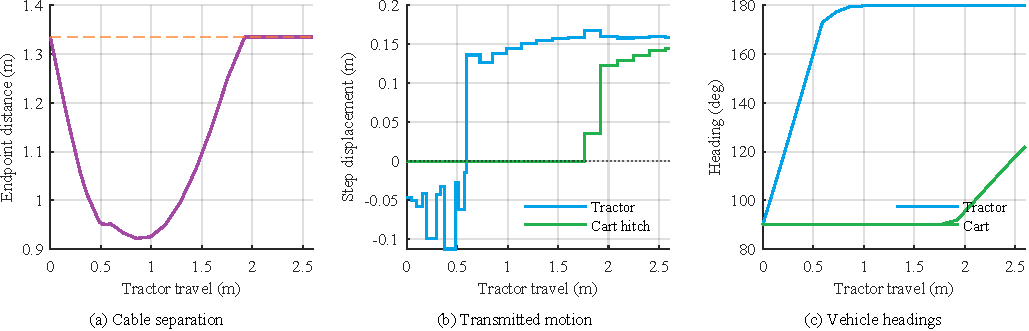
\includegraphics[width=\textwidth]{mode_evidence.pdf}
\caption{Cable distance, transmitted displacement, and vehicle headings during initial tractor repositioning.}
\label{fig:modes}
\end{figure*}

\begin{table*}[!t]
\centering\caption{Four-run sensitivity to numerical termination and process timing}
\label{tab:repeat}
\footnotesize\begin{tabular}{llrrrr}
\toprule
Case & Method & New & Objective range & $t_{50}$ (s) & IQR (s)\\
\midrule
W02 & Proposed & 4/4 & 16.99--17.00 & 30.77 & 0.18\\
W02 & MAX & 4/4 & 18.80--18.80 & 31.00 & 0.85\\
W05 & Proposed & 4/4 & 13.09--13.09 & 31.14 & 0.29\\
W05 & MAX & 4/4 & 13.13--13.13 & 30.71 & 0.02\\
W09 & Proposed & 4/4 & 31.17--31.24 & 32.99 & 0.63\\
W09 & MAX & 4/4 & 30.98--30.98 & 34.13 & 0.07\\
\bottomrule\end{tabular}
\end{table*}

Table~\ref{tab:repeat} includes the primary run and three additional runs on each fixed instance, measuring sensitivity to numerical termination and process timing. The task-dependent quality ordering persists: the proposed method has lower objectives on W02 and W05, while MAX has lower objectives on W09.

Repeated runs use the same three predeclared cases W02, W05, and W09, with three additional runs per method and case. They measure sensitivity to timing and numerical termination on fixed instances. An auxiliary LSE test changes only the mode expression of MAX at inverse scales $100$ and $1000$ m$^{-1}$ on those same cases. Its pointwise excess above a direct maximum is bounded by $\log 2/\rho$, where $\rho$ is the inverse scale, and it can transmit nonzero displacement while slack. Every smoothed output is checked against the exact cable relation.
The LSE variants return 0/3 and 0/3 outputs that pass the exact common validator at inverse scales 100 and 1000, respectively. They improve the common seed in 0/3 and 0/3 cases. These outcomes are evaluated under the exact cable relation rather than the smoothed surrogate. The final planner retains the direct maximum.


Figure~\ref{fig:budgets} varies the nominal allowance over 15, 30, and 60 s on W02, W05, and W09. It reports mean per-case travel reduction and newly validated outputs for Proposed, MAX, and MINLP. The horizontal coordinate of the quality plot is measured median backend time, including overhead; the acceptance plot uses the nominal allowance. All runs retain the same models, seeds, and acceptance rules. Longer allowances need not improve a nonconvex solve monotonically because they can change the intermediate candidates and time available for restoration.
At the 15-s allowance, Proposed and MAX produce 3/3 and 2/3 new validated outputs, with mean travel reductions of 4.27\% and 0.99\%. At the 60-s allowance, the corresponding median measured times are 38.95 and 61.20 s, and the mean travel reductions are 4.55\% and 1.45\%. These results describe the three fixed budget-test tasks.

\begin{figure*}[!t]
\centering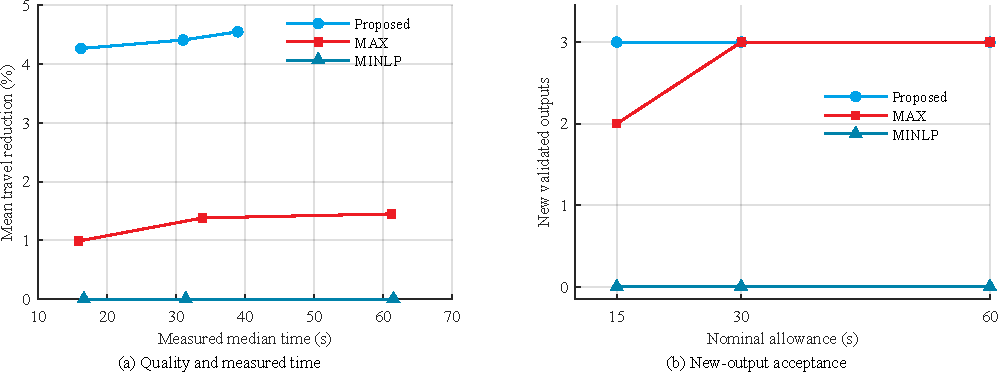
\includegraphics[width=\textwidth]{budget_sensitivity.pdf}
\caption{Quality and new-output acceptance under three nominal computation allowances on three fixed tasks.}
\label{fig:budgets}
\end{figure*}

\subsection{Footprint Variations and a Serial Formation}
Five cart geometries share the unchanged W02 warehouse, goal, cable length, kinematics, mesh, and initial controls. Only the cart polygon changes. S01--S05 respectively denote a nominal rectangle, compact rectangle, long narrow rectangle, irregular pentagon, and wide hexagon. Their actual vertices generate the OBCA halfspaces. Both planners use the same seed for each shape, checked before optimization.
\begin{table}[!tb]
\centering\caption{Five cart footprints on W02}
\label{tab:shapes}
\footnotesize\begin{tabular}{llrrr}
\toprule
Case & Extents (m) & New & $J_{\rm prop}$ & $J_{\rm MAX}$\\
\midrule
S01 & $1.05\times1.10$ & 1/1 & 17.00 & 18.80\\
S02 & $0.90\times0.70$ & 1/1 & 18.24 & 18.82\\
S03 & $1.25\times0.90$ & 1/1 & 16.54 & 18.80\\
S04 & $1.05\times1.10$ & 1/1 & 17.00 & 18.81\\
S05 & $1.05\times1.20$ & 1/1 & 17.05 & 18.70\\
\bottomrule\end{tabular}
\end{table}

All five footprints share the unchanged W02 map, task, and initial controls. The proposed method returns 5/5 new validated trajectories, compared with 5/5 for MAX. The actual polygon halfspaces are used throughout optimization and independent validation.
In Table~\ref{tab:shapes}, New entries report Proposed/MAX acceptance; both objectives are recomputed from the returned controls.


\begin{figure*}[!t]
\centering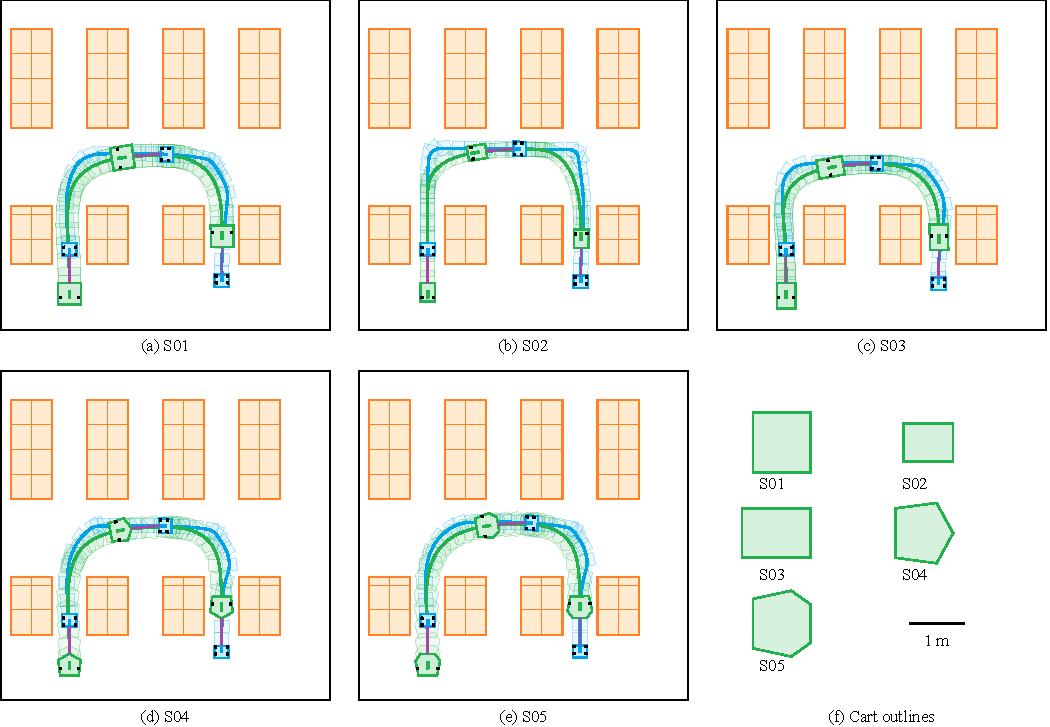
\includegraphics[width=.915\textwidth]{shape_trajectories.pdf}
\caption{Five convex cart geometries planned in the unchanged shape-test warehouse.}
\label{fig:shapes}
\end{figure*}

The serial example connects three passive carts with individual convex footprints and rear attachment points. Recursive application of~\eqref{eq:serial} produces a constructive route through another $16\times16$ m rack environment. Body separation, endpoint lengths, and nonreversing conditions are checked at every replay substep. Cable routes are checked at the original control boundaries and the corresponding boundary configurations from finer integration. This example evaluates serial kinematic feasibility. Figure~\ref{fig:train} shows the occupied route and two maneuver configurations.
The three-cart construction passes the recursive kinematic and geometric checks, with minimum body clearances of 0.178 m on the original grid and 0.204 m on finer replay. This constructive demonstration extends the prescribed per-node cable-routing model to serial towing. Physical multi-cart operation additionally requires continuous cable handling and cable--cable interaction assessment.


\begin{figure*}[!t]
\centering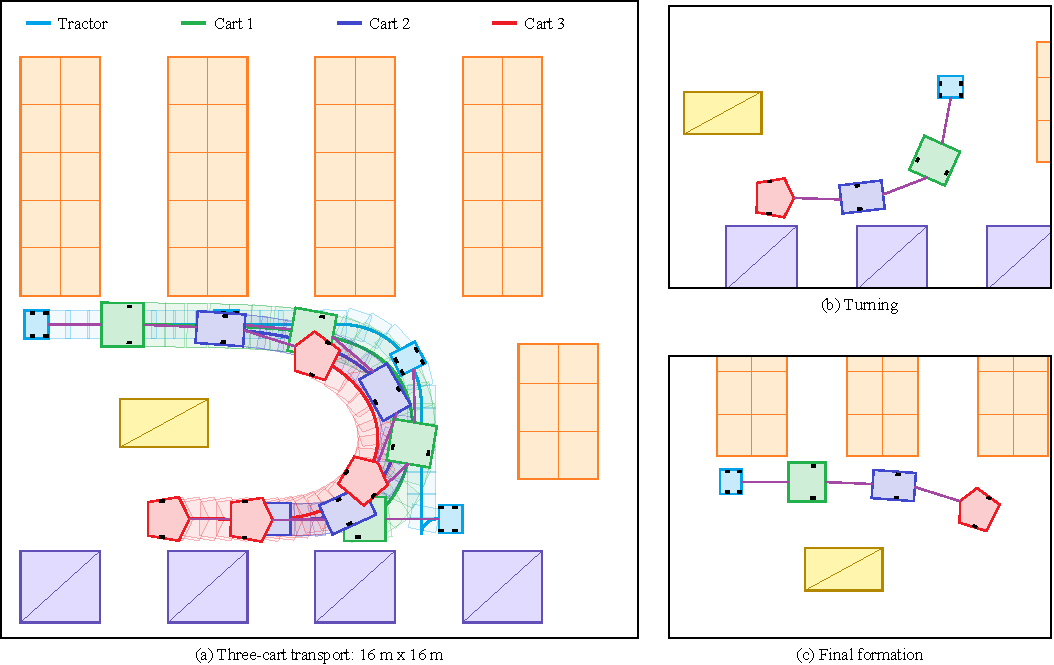
\includegraphics[width=.915\textwidth]{train_extension.pdf}
\caption{A three-cart formation navigating a confined square warehouse with individual convex footprints.}
\label{fig:train}
\end{figure*}

\FloatBarrier
\section{Conclusion}
Optimization-based motion planning exploits cable slack to reposition an autonomous tractor around a waiting cart. For an equal-length rigid drawbar, a geometric theorem excludes reorientation in a specified strip family; 18 corresponding cable maneuvers satisfy the proposed discrete kinematics and geometric cable-routing checks. Under the quasistatic stopping and hitch-mobility assumptions, the formulation unifies unilateral transmission, convex body geometry, and recursive serial towing. Feasible control restoration, replay-guided reserves, and final recovery together improve feasible-seed refinement: the nine warehouse tasks yield 4.36\% mean travel reduction, compared with 1.07\% for direct MAX with recovery, with new validated outputs in all nine cases for both. Convex footprint variations and a three-cart construction illustrate geometric and structural flexibility. The framework supports trajectory preparation before warehouse task execution. Physical validation will address stopping behavior, continuous cable interaction, and closed-loop tracking.
\IEEEtriggeratref{8}
\bibliographystyle{IEEEtran}
\bibliography{references}
\end{document}
